% !TEX program = xelatex
% 5-minute beamer slides for 第二届"良文杯" finals
% Team 792 "超级回天什么时候上映" — 史景喆 (清华大学)
% Public LB #1 / Private LB #1
%
% Note: Coding Agent section is intentionally OUT of scope.

\documentclass[aspectratio=169,11pt]{beamer}

% ---------- Fonts (CJK via xeCJK) ----------
\usepackage{fontspec}
\usepackage{xeCJK}
\setCJKmainfont[BoldFont={Noto Serif CJK SC Bold}]{Noto Serif CJK SC}
\setCJKsansfont[BoldFont={Noto Sans CJK SC Bold}]{Noto Sans CJK SC}
\setCJKmonofont{Noto Sans Mono CJK SC}
\setmainfont{Nimbus Roman}[
  Extension={.otf},
  Path=/usr/share/fonts/opentype/urw-base35/,
  UprightFont=NimbusRoman-Regular,
  BoldFont=NimbusRoman-Bold,
  ItalicFont=NimbusRoman-Italic,
  BoldItalicFont=NimbusRoman-BoldItalic,
]

% ---------- Theme + colors ----------
\usetheme{default}
\useinnertheme{rounded}
\useoutertheme{infolines}
\setbeamertemplate{navigation symbols}{}

\definecolor{icmlblue}{RGB}{0,30,90}
\definecolor{lblue}{RGB}{40,120,210}
\definecolor{accred}{RGB}{170,0,0}
\definecolor{lightgray}{RGB}{238,238,238}

\setbeamercolor{frametitle}{fg=icmlblue}
\setbeamercolor{title}{fg=icmlblue}
\setbeamercolor{author}{fg=black!70}
\setbeamercolor{institute}{fg=black!70}
\setbeamercolor{date}{fg=black!70}
\setbeamercolor{structure}{fg=icmlblue}
\setbeamercolor{itemize item}{fg=icmlblue}
\setbeamercolor{itemize subitem}{fg=lblue}
\setbeamercolor{footline}{fg=black!60}
\setbeamerfont{frametitle}{series=\bfseries,size=\large}
\setbeamerfont{footline}{size=\tiny}

% kill the default nav bar in infolines, keep just author / title / pages
\setbeamertemplate{footline}{%
  \leavevmode%
  \hbox{%
    \begin{beamercolorbox}[wd=.34\paperwidth,ht=2.25ex,dp=1ex,leftskip=1.2ex]{author in head/foot}%
      \scriptsize 队伍 792 · 超级回天什么时候上映 · 史景喆（清华）%
    \end{beamercolorbox}%
    \begin{beamercolorbox}[wd=.5\paperwidth,ht=2.25ex,dp=1ex,center]{title in head/foot}%
      \scriptsize 良文杯 2026 决赛 ·\ 公榜\,\#1\,·\,私榜\,\#1%
    \end{beamercolorbox}%
    \begin{beamercolorbox}[wd=.16\paperwidth,ht=2.25ex,dp=1ex,rightskip=1.2ex]{date in head/foot}%
      \hfill\scriptsize \insertframenumber{}\,/\,\inserttotalframenumber%
    \end{beamercolorbox}}%
  \vskip0pt%
}

% remove headline (infolines section bar) since we have no sections
\setbeamertemplate{headline}{}

% ---------- Packages ----------
\usepackage{amsmath}
\usepackage{amssymb}
\usepackage{graphicx}
\usepackage{booktabs}
\usepackage{array}
\usepackage{tabularx}
\usepackage{tikz}
\usepackage{xcolor}
\usepackage{pifont}

% ---------- Highlight macro (matches onepage \hl) ----------
\newcommand{\hl}[1]{\textcolor{lblue}{\textbf{#1}}}
\newcommand{\rhl}[1]{\textcolor{accred}{\textbf{#1}}}
\newcommand{\sn}[1]{\textsuperscript{\tiny #1}}

% tight itemize
\setbeamertemplate{itemize item}{\raisebox{0.18ex}{\scalebox{0.7}{\(\blacktriangleright\)}}}
\setbeamertemplate{itemize subitem}{\raisebox{0.18ex}{\scalebox{0.6}{\(\bullet\)}}}

\title{\bfseries 面向 PnL 目标的 LOB 中间价方向预测}
\subtitle{$\Delta$mid 回归\,$+$\,SPO+ 决策焦点学习\,$+$\,$50\!\times\!50$ 异质集成}
\author{史景喆\,\,\,\, 清华大学}
\institute{\small 队伍 \textbf{792}\,:\,\,\,超级回天什么时候上映}
\date{\small 第二届"良文杯"统计建模与 AI 预测挑战赛\,·\,决赛汇报}

\begin{document}

% =========================================================
% Slide 1 — Title
% =========================================================
\begin{frame}[plain]
  \vfill
  \begin{center}
    {\Large\bfseries\color{icmlblue} 面向 PnL 目标的 LOB 中间价方向预测}\\[6pt]
    {\large $\Delta$mid 回归 \,$+$\, SPO+ 决策焦点学习 \,$+$\, $50\!\times\!50$ 异质集成}\\[18pt]

    
\begin{tikzpicture}
      \draw[lblue, line width=1.2pt] (0,0) -- (8,0);
    \end{tikzpicture}\\[10pt]

    {\large \textbf{史景喆}\,\, 清华大学}\\[4pt]
    {\small 队伍随机码 \textbf{792}\,\,\textbar\,\,队伍：\textbf{超级回天什么时候上映}}\\[18pt]

    \begin{tikzpicture}
      \node[draw=icmlblue, line width=0.9pt, fill=icmlblue!5,
            inner sep=8pt, rounded corners=3pt] {
        \begin{minipage}{0.78\textwidth}
          \centering
          \large
          公榜 $-6.65 \to$ \rhl{$+35.64$}\,\, （baseline 之上增益 \rhl{$+42.29$}）\\[3pt]
          \textbf{公榜 \#1\,\,\textbar\,\,私榜 \#1}（$h{=}60$）\,\textbar\,\, $h{=}40$ 私榜亦第一
        \end{minipage}
      };
    \end{tikzpicture}

    \vspace{12pt}
    {\footnotesize 第二届"良文杯"统计建模与 AI 预测挑战赛 · 决赛汇报}
  \end{center}
  \vfill
\end{frame}

% =========================================================
% Slide 2 — Problem & Scoring
% =========================================================
\begin{frame}{Problem 与评分 —— 这是一道带交易成本的「期望收益预测」题}
  \begin{columns}[T,onlytextwidth]
    \column{0.50\textwidth}
    \textbf{\color{icmlblue}数据}
    \begin{itemize}\setlength{\itemsep}{2pt}
      \item 5 只匿名 A 股 $\times$ 120 交易日 $\times$ 4002 ticks (3 秒/tick)
      \item 154 维原始字段：OHLC / \textbf{10 档 LOB} / \textbf{6 类订单流}（intst, ind, acc）/ 衍生 spread \& imbalance
      \item 1200 parquet, $\sim$474 MB; 8 文件涨停日深档 ask 含少量 NaN（pipeline \texttt{isfinite} 兜底）
    \end{itemize}
    \vspace{4pt}
    \textbf{\color{icmlblue}评分}
    \begin{itemize}\setlength{\itemsep}{2pt}
      \item 动作 $\hat a\!\in\!\{0,1,2\}$, 仅买/卖扣 $\sim\!0.02\%$ 双边手续费
      \item 总分 $\mathrm{Score}=\max_{h\in\{5,10,20,40,60\}}\sum_i\mathrm{pnl}_i^{(h)}$
      \item \hl{本文以 $h{=}60$ 为主线}
    \end{itemize}

    \column{0.46\textwidth}
    \begin{block}{\color{accred}评测端 3 条硬约束（违反 = 0 分）}
      \scriptsize
      \begin{enumerate}\setlength{\itemsep}{2pt}
        \item \textbf{\texttt{date} 被置 0}\,\,---\,\,不能当 feature
        \item \textbf{测试点顺序被打乱}\,\,---\,\,Predictor 无跨调用 state
        \item \textbf{sym 0--4 可能含训练外股票}\,\,---\,\,模型必须 \textbf{sym-agnostic}：不用 sym embedding / per-sym 归一化 / per-sym 模型
      \end{enumerate}
    \end{block}
    \vspace{4pt}
    {\footnotesize\itshape 这 3 条约束塑造了所有后续设计 —— 特别是 \hl{window-$z$} 归一化与 \hl{simple-mean 集成}。}
  \end{columns}
\end{frame}

% =========================================================
% Slide 3 — Pipeline overview
% =========================================================
\begin{frame}{方案 Pipeline 一览}
  \vspace{-2pt}
  \begin{center}
    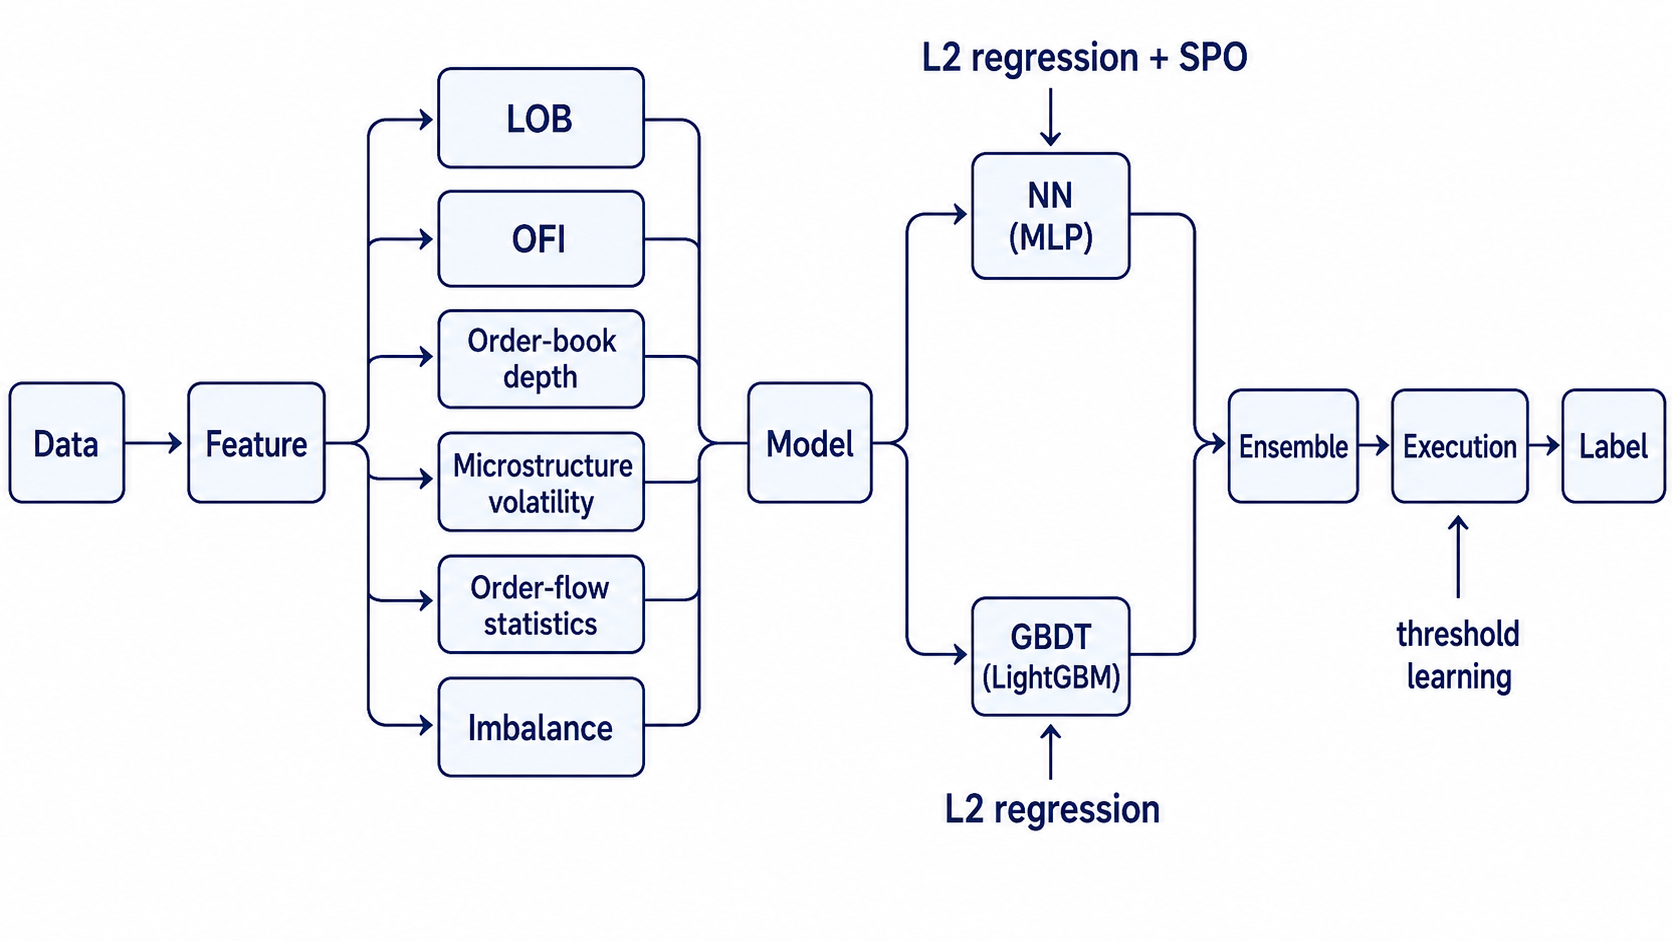
\includegraphics[width=0.82\linewidth,height=0.70\textheight,keepaspectratio]{Pipeline_Img.png}
  \end{center}
  \vspace{-4pt}
  \begin{center}\footnotesize
  Data $\to$ \hl{6 家族 Feature (359 维)} $\to$ \hl{NN(MLP) + LGB(L2 回归)} 异质 Model
  $\to$ Ensemble $\to$ Execution (\hl{ETUD 阈值学习}) $\to$ Label
  \end{center}
\end{frame}

% =========================================================
% Slide 4 — Feature families
% =========================================================
\begin{frame}{因子工程：六大家族 —— F1 + F3 占 LGB gain 75.5\%}
  \vspace{-2pt}
  \begin{center}
    
\includegraphics[width=0.95\linewidth,height=0.70\textheight,keepaspectratio]{Feature_Img.pdf}
  \end{center}
  \vspace{-4pt}
  \begin{columns}[T,onlytextwidth]
    \column{0.62\textwidth}
    \scriptsize
    \begin{itemize}\setlength{\itemsep}{-1pt}\setlength{\topsep}{0pt}\setlength{\parsep}{0pt}
      \item \hl{F1 LOB 派生 (40.4\% gain)}\,:\,\,10 档报价/挂单量 + WMP + spread
      \item \hl{F3 订单流强度 (35.1\% gain)}\,:\,\,\texttt{ma/mb/la/lb\_intst} + EWMA
    \end{itemize}
    \column{0.36\textwidth}
    \scriptsize\itshape
    Top-10 因子全在 F1+F3；F5 与其它族 $|\rho|\!\le\!0.07$，\textbf{正交补强}。
  \end{columns}
\end{frame}

% =========================================================
% Slide 5 — Three preprocessing tricks
% =========================================================
\begin{frame}{三类关键预处理 —— window-$z$ 单 trick 拉高 +22.88}
  \begin{columns}[T,onlytextwidth]
    \column{0.33\textwidth}
    \begin{block}{\hl{window-$z$ score}}
      \scriptsize
      所有统计量在 \textbf{100-tick 切片内}自适应归一化\\[2pt]
      \,\,$\Rightarrow$ 跨 stock 分布差异被窗口吸收\\[2pt]
      \,\,$\Rightarrow$ 训练外股票也能 zero-shot
      \begin{center}
        \vspace{2pt}
        \rhl{$+22.88$ PnL}\\
        \scriptsize{(单 trick 最大跃升)}
      \end{center}
    \end{block}
    \column{0.33\textwidth}
    \begin{block}{\hl{买卖镜像数据增强}}
      \scriptsize
      训练样本与 bid$\leftrightarrow$ask 互换 $+$ 标签反转的镜像拼接\\[2pt]
      \,\,$\Rightarrow$ 训练集 $\times 2$\\[2pt]
      \,\,$\Rightarrow$ 强制方向\textbf{对称先验}
      \begin{center}
        \vspace{6pt}
        \rhl{$+2.41$ PnL}
      \end{center}
    \end{block}
    \column{0.33\textwidth}
    \begin{block}{\hl{稳健归一化 (sign-log1p)}}
      \scriptsize
      \texttt{amount\_delta} 量级 $10^3$--$10^6$\,，重尾压制：
      \[
        v\mapsto\operatorname{sign}(v)\log(1{+}|v|)
      \]
      \,\,$\Rightarrow$ NN/LGB 梯度数值稳定\\[3pt]
      \,\,$\Rightarrow$ LGB 大幅受益, NN 中性
      \begin{center}
        \vspace{2pt}
        \scriptsize\itshape (与 F5/F6 一同贡献)
      \end{center}
    \end{block}
  \end{columns}
  \vspace{6pt}
  \begin{center}
    \footnotesize\itshape
    共同主题：\textbf{在输入侧让模型"看不见"非平稳分布偏移}，这是 OOD 上能稳的根本。
  \end{center}
\end{frame}

% =========================================================
% Slide 6 — Models: NN + LGB heterogeneous
% =========================================================
\begin{frame}{模型工程：异质 NN $+$ LGB —— 故意不用 RNN/Transformer/CNN}
  \begin{columns}[T,onlytextwidth]
    \column{0.48\textwidth}
    \begin{block}{\hl{NN}\,\, : 4-layer MLP}
      \scriptsize
      $[359\to 256\to 128\to 64\to 1]$\,\, ($\sim$120k 参数)\\
      LayerNorm $+$ GELU $+$ Dropout\\[2pt]
      \textbf{LayerNorm 走样本级}\,\,$\Rightarrow$ 避免 batch 内污染\\[3pt]
      \textit{为什么不用更复杂架构？}\\
      \scriptsize\color{black!70}
      window-$z$ + 6 家族派生已经把 100-tick 时序信息蒸馏成静态因子，\\
      RNN/Transformer/CNN 容易 in-sample 膨胀，OOD 反而退化。
    \end{block}

    \column{0.48\textwidth}
    \begin{block}{\hl{LGB}\,\, : L2 $\Delta$mid 回归}
      \scriptsize
      \texttt{objective = regression\_l2}\\
      目标 $y = (\mathrm{mp}_{t+60}-\mathrm{mp}_t)/(\mathrm{mp}_t+1)$\\[3pt]
      \textbf{class-balanced 样本权重}\,\,(h=60 三类频率倒数)\\
      \,\,$\Rightarrow$ 稀疏涨/跌样本得到更高梯度\\[3pt]
      \textit{为什么 L2 而不是 3-class CE？}\\
      \scriptsize\color{black!70}
      回归保留连续置信度,\\ETUD 阈值层可在执行侧二次决策；分类把信息提前 collapse。
    \end{block}
  \end{columns}
  \vspace{6pt}
  \begin{center}\small
    族内 simple mean，跨族固定权重 \hl{$\mathrm{LGB}:\mathrm{NN}=1.5:1$}（GBDT 在表格数据上略强 $\Rightarrow$ 略重）
  \end{center}
\end{frame}

% =========================================================
% Slide 7 — SPO+ DFL
% =========================================================
\begin{frame}{训练核心：SPO+ 决策焦点学习 —— 把梯度对齐离散动作的期望收益}
  \vspace{-4pt}
  \begin{columns}[T,onlytextwidth]
    \column{0.55\textwidth}
    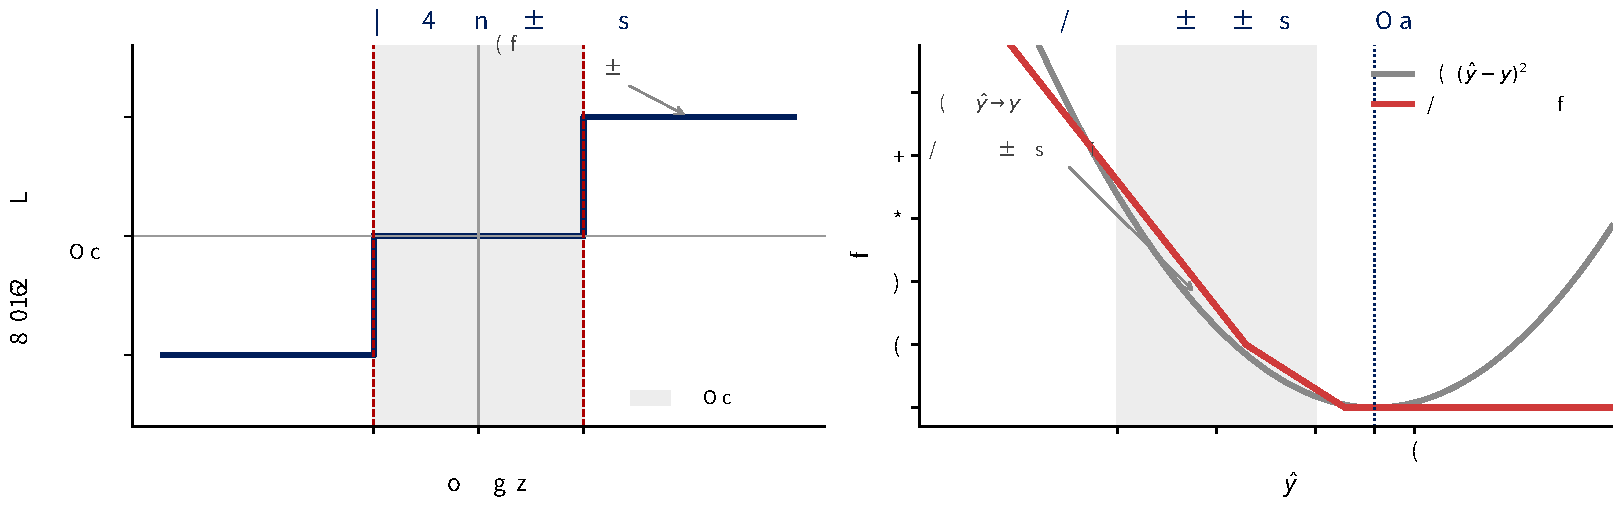
\includegraphics[width=\linewidth]{spo_intuition.pdf}

    \column{0.45\textwidth}
    \scriptsize
    \textbf{\color{icmlblue}核心问题：}\\
    L2 回归追真值，但评分只关心\textbf{动作 $\hat a$ 是否越过费率门槛 $f$}\,。\\[4pt]
    \textbf{\color{icmlblue}SPO+ surrogate (Elmachtoub \& Grigas 2022)：}
    \[
      \ell_{\mathrm{SPO+}} = \mathrm{ReLU}\!\big(|2\hat y{-}y|{-}f\big) - z^{\!\star}(y)(2\hat y{-}y) + f|z^{\!\star}(y)|
    \]
    \[
      L = (\hat y-y)^2 + \lambda\,\ell_{\mathrm{SPO+}},\,\, \lambda{=}30
    \]
    \vspace{2pt}
    \textbf{\color{icmlblue}两阶段：}
    \begin{itemize}\setlength{\itemsep}{1pt}
      \item Phase 1 — pure L2 回归预训练
      \item Phase 2 — warm-start 联合 L2 $+$ SPO+ 微调 (lr $3{\times}10^{-5}$, 11 ep)
    \end{itemize}
    \vspace{2pt}
    \rhl{$+3.54$ PnL}（最大单一训练 trick 增益）
  \end{columns}
\end{frame}

% =========================================================
% Slide 8 — Ensemble + Execution
% =========================================================
\begin{frame}{集成 \& 执行：$50\!\times\!50$ simple-mean $+$ ETUD 非对称阈值}
  \begin{columns}[T,onlytextwidth]
    \column{0.52\textwidth}
    \begin{block}{\hl{50 NN $+$ 50 LGB 异质集成}}
      \scriptsize
      5 组 HP $\times$ 10 seed = 50 NN + 50 LGB\\
      \textbf{simple mean，不学权重}\\[3pt]
      为什么？\\
      \,\,$\bullet$ NN--NN avg $|\rho|=0.93$，LGB--LGB $0.84$\\
      \,\,$\bullet$ 设计矩阵条件数 $5.4{\times}10^{4}$（病态共线）\\
      \,\,$\bullet$ bounded NNLS 本地涨,\,公榜 \rhl{$-4.64$}\\[3pt]
      \textbf{OOD 上 simple mean 是稳健最优}
    \end{block}

    \column{0.45\textwidth}
    \begin{block}{\hl{ETUD —— 非对称执行阈值}}
      \scriptsize
      \vspace{-4pt}
      \[
      \hat a =
      \begin{cases}
        +1\,(\text{买}), & \hat y > +\theta_{\mathrm{up}}\\
        -1\,(\text{卖}), & \hat y < -\theta_{\mathrm{dn}}\\
        \phantom{+}0, & \text{otherwise}
      \end{cases}
      \]
      \vspace{-2pt}
      $\theta_{\mathrm{up}}{=}3.00{\times}10^{-4}$\\
      $\theta_{\mathrm{dn}}{=}2.16{\times}10^{-4}$\\[3pt]
      由验证集 \textbf{2D DE 搜出后冻结}\\
      不对称匹配训练样本正向漂移
    \end{block}
  \end{columns}
  \vspace{4pt}
  \begin{center}\small\itshape
    决策参数\textbf{不在 OOF 上学权重}\,，只在执行侧用 1 个二维阈值搜——这是 OOD 上"简单 = 稳健"的延伸。
  \end{center}
\end{frame}

% =========================================================
% Slide 9 — Big ablation waterfall
% =========================================================
\begin{frame}{大消融 waterfall —— 从 $+0.52$ 到 $+41.58$ 的 9 步关键跳跃}
  \begin{center}
    \vspace{-2pt}
    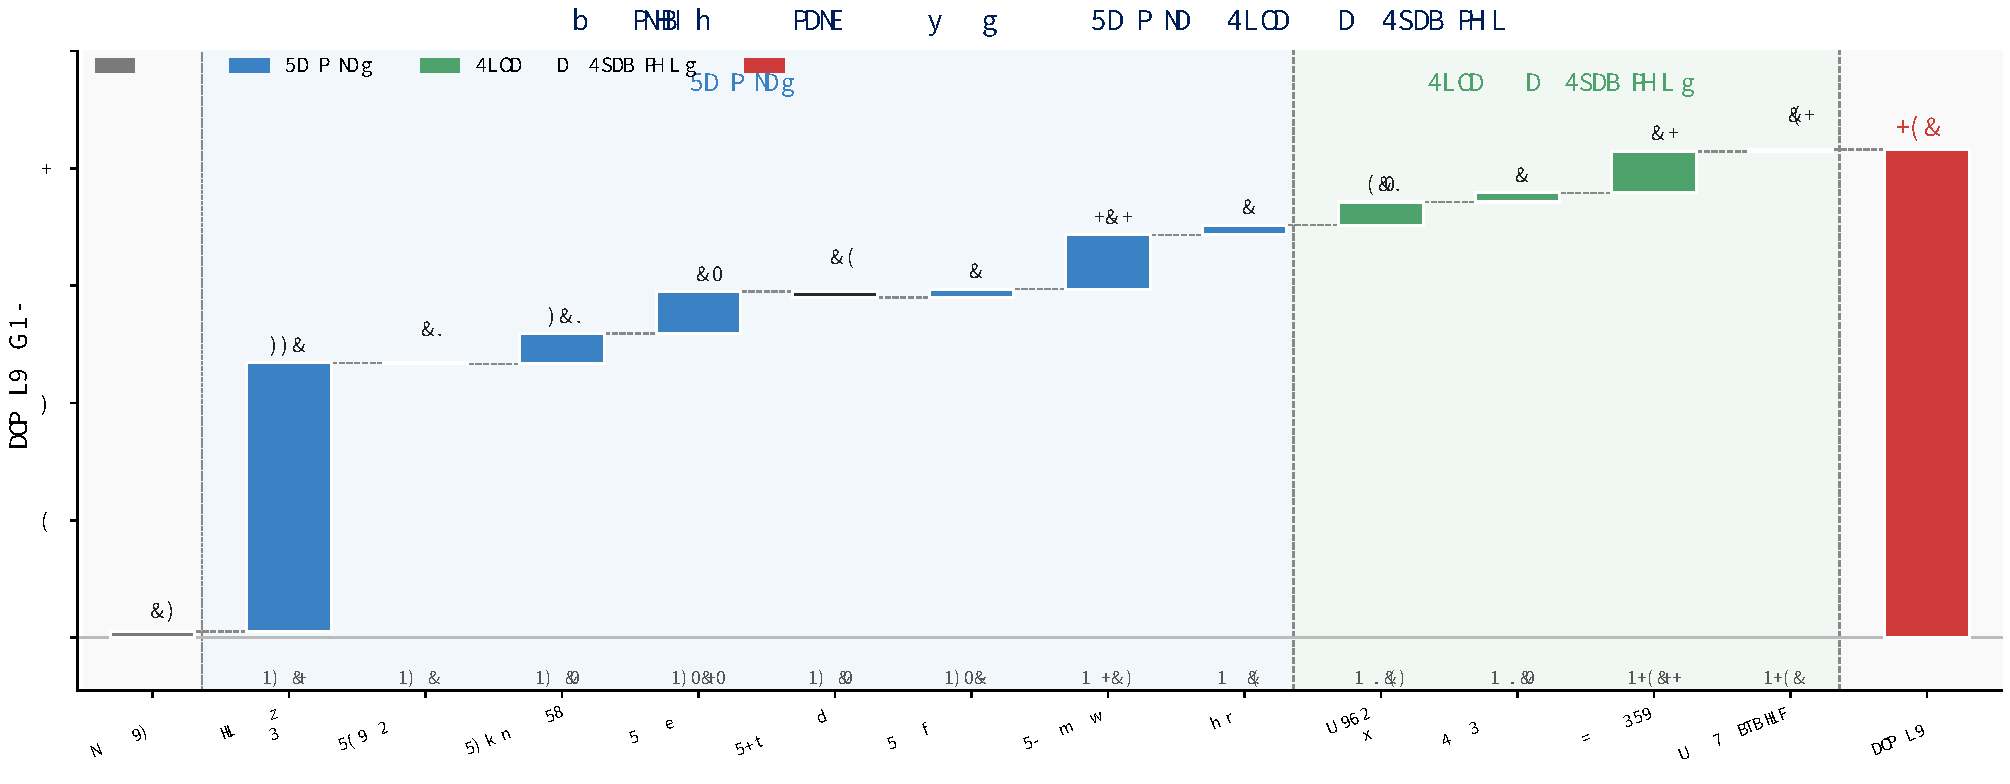
\includegraphics[width=0.98\linewidth]{waterfall.pdf}
  \end{center}
  \vspace{-6pt}
  \begin{center}\scriptsize
    \textbf{3 个高 ROI trick}\,\,：\hl{window-$z$ +22.88}（输入侧 OOD）\,·\,\hl{SPO+ DFL +3.54}（训练侧决策对齐）\,·\,\hl{F6 不对称性 +4.64}（因子）
  \end{center}
\end{frame}

% =========================================================
% Slide 10 — Leaderboard
% =========================================================
\begin{frame}{Leaderboard —— 公榜 \#1 / 私榜 \#1 / $h{=}40$ 私榜亦第一}
  \vspace{-4pt}
  \begin{center}
    \setlength{\tabcolsep}{6pt}\renewcommand{\arraystretch}{1.15}
    \small
    \begin{tabular}{@{}lcccccc@{}}
      \toprule
      榜单 & $h$ & 准确率 & 召回率 & F$_{0.5}$ & 单次收益率 & \textbf{累计收益率 (评分)} \\
      \midrule
      \textbf{公榜} & 60 & 0.3233 & 0.3177 & 0.3222 & $1.91{\times}10^{-4}$ & \rhl{\textbf{35.64}}\,\,(\textbf{\#1}) \\
      \textbf{私榜} & 60 & 0.3122 & 0.3390 & 0.3172 & $2.39{\times}10^{-4}$ & \rhl{\textbf{41.61}}\,\,(\textbf{\#1}) \\
      \textbf{私榜} & 40 & 0.2712 & 0.4062 & 0.2905 & $1.94{\times}10^{-4}$ & \rhl{\textbf{38.65}}\,\,(\textbf{$h{=}40$ 第一}) \\
      \bottomrule
    \end{tabular}
  \end{center}
  \vspace{6pt}
  \begin{columns}[T,onlytextwidth]
    \column{0.55\textwidth}
    \footnotesize
    \begin{itemize}\setlength{\itemsep}{2pt}
      \item 本文研究主线 $h{=}60$，模型/损失/特征/阈值\textbf{全部围绕 $h{=}60$ 优化}
      \item $h{<}60$ 不重新训练、不重新调参\,，只按 $\sqrt{h/60}$ 简单缩放阈值
      \item 即便如此 $h{=}40$ 仍取该 horizon 第一（$+38.65$）
    \end{itemize}
    \column{0.42\textwidth}
    \footnotesize\itshape
    \,\,准确率/召回率/F$_{0.5}$ 针对涨/跌出手类 (label$\in\{0,2\}$)\,，\\
    \,\,"不出手"不计；评分 $=$ 累计收益率。
  \end{columns}
\end{frame}

% =========================================================
% Slide 11 — Takeaways
% =========================================================
\begin{frame}{Takeaways —— 5 条对未来 LOB 实盘有迁移价值的经验}
  \vspace{2pt}
  \begin{enumerate}\setlength{\itemsep}{6pt}
    \item \hl{sym-agnostic 是硬约束，不是"建议"}\,\,---\,\,任何 sym embedding / per-sym 归一化 / per-sym 模型都会被评测端打散。\textbf{在输入侧（window-$z$）解决，比在模型侧绕路简单 10 倍}。

    \item \hl{决策焦点学习给 $+3.54$ PnL}\,\,---\,\,把 L2 回归改 SPO+ 决策焦点 surrogate，让梯度真正对齐执行端的离散动作期望收益。\textbf{评分函数本身就是 loss，最好的 loss 是 surrogate of scoring}。

    \item \hl{OOD 上 simple mean $>$ learned weights}\,\,---\,\,基模型平均 corr 0.84/0.93、设计矩阵病态共线下，bounded NNLS 本地涨而公榜 $-4.64$。\textbf{决策参数不要在 OOF 上学}。

    \item \hl{F1 + F3 = 75.5\% 的 LGB gain}\,\,---\,\,LOB 派生 + 订单流强度是绝大多数 alpha 的载体；F2/F4/F5/F6 是\textbf{方差源去相关而非均值源}。

    \item \hl{窗口 + 镜像 + 稳健归一化}\,\,---\,\,三个看似"小"的预处理一起，把 NN 从 $+0.52$ 抬到 $+34$；\textbf{特征工程的复利远超模型架构选择}。
  \end{enumerate}
\end{frame}

% =========================================================
% Slide 12 — Closing
% =========================================================
\begin{frame}[plain]
  \vfill
  \begin{center}
    {\Large\bfseries\color{icmlblue} 谢谢评委 \& 良文杯组委会}\\[18pt]

    
\begin{tikzpicture}
      \draw[lblue, line width=1.2pt] (0,0) -- (8,0);
    \end{tikzpicture}\\[14pt]

    \begin{tabular}{rl}
      \small 累计收益率 (公榜)：& \rhl{\large $+35.64$}\,\,（\textbf{\#1}）\\
      \small 累计收益率 (私榜)：& \rhl{\large $+41.61$}\,\,（\textbf{\#1}）\\
      \small 起点 baseline：& \small $-6.65$\,\,$\Rightarrow$\,\,净增益 \rhl{$+42.29$}\\
    \end{tabular}\\[18pt]

    {\small 队伍 \textbf{792} ·\,\,超级回天什么时候上映\,\,· \,\,史景喆（清华大学）}\\[6pt]
    {\footnotesize\itshape 代码开源\,:\,\,\texttt{github.com/JingzheShi/liangwenbei}}
  \end{center}
  \vfill
  \begin{center}\tiny\color{black!55}
    References:\,\, Cont \& Kukanov (2014) OFI\,\,·\,\,Stoikov (2014) WMP\,\,·\,\,Elmachtoub \& Grigas (2022) SPO+\,\,·\,\,Gorishniy et al.\ (2021) FT-Transformer
  \end{center}
\end{frame}

\end{document}
